%
\hsection{pip and Virtual Environments}%
\label{sec:pipAndVenv}%
%
The go-to tool for installing \python\ \pglspl{package} is \pip~\cite{PSF2024IPM,PD2024PD}.%
%
\usefulTool{pip}{%
\pip\ is a software that can be used to install \pglspl{package} under \python. %
\begin{itemize}%
\item With the command \bashil{pip install thePackage}, the \pgls{package}~\bashil{thePackage} is installed.%
\item With the command \bashil{pip install "thePackage==version"}, the version~\bashil{version} of the \pgls{package}~\bashil{thePackage} is installed.%
\item With the command \bashil{pip install -r requirements.txt}, the \pglspl{package} listed in the requirements file \textil{requirements.txt} are installed. %
A requirements file allows to put multiple package/version dependencies that would otherwise command line arguments of \pip\ into a single file~\cite{PD2024RFF}.%
\end{itemize}%
%
\pip\ should always be used in a \pgls{virtualEnvironment}, see~\cref{bp:venvInstall,bp:pipVenv}.%
}%
%
The standard way to install \pglspl{package} for use with \python\ is in a so-called \pgls{virtualEnvironment}.
A \pgls{virtualEnvironment} is a directory with an isolated \python\ installation and \pgls{package} directory~\cite{PSF2024VEAP,PEP405}.
Multiple separate \pglspl{virtualEnvironment} can exist on a computer, all with their own set of installed \pglspl{package}.
This allows you to have different \python\ setups for different applications by installing them into different \pglspl{virtualEnvironment}.
\Pglspl{virtualEnvironment} are particularly useful if different applications need different versions of the same \pglspl{package}.
This way, version clashes are avoided.
They also give you better understanding about the actual dependencies of your applications:
Installing the \pglspl{package} directly needed by an application into a new \pgls{virtualEnvironment} will also install their dependencies and the dependencies of their dependencies, and so on.%
%
\bestPractice{venvInstall}{%
\Pglspl{package} should \emph{always} be installed in \pglspl{virtualEnvironment} and never system-wide (maybe with the exception of \pip\ and \venv).%
}%
%
\bestPractice{pipVenv}{\sloppy%
The command \bashil{pip install} should always be used with the option \bashil{--require-virtualenv}, e.g., \bashil{pip install --require-virtualenv thePackage}. %
This enforces that \pip\ is really executed in a \pgls{virtualEnvironment} and will cause an error otherwise.%
}%
%
\usefulTool{venv}{The module \venv\ is used for creating and managing \pglspl{virtualEnvironment} under \python.}%
%
%
\gitPython{\programmingWithPythonCodeRepo}{10_packages/numpy_user.py}{--args format}{packages:numpy_user}{%
A small \python\ script using the \numpy\ library.}%
%
For demonstration purposes, let us assume that we have written a program using the \pgls{package} \numpy~\cite{HMvdWGVCWTBSKPHvKBHFdRWPGMSRWAGO2020APWN,DBvR2024ITN,J2018NPSCADSAWNSAM}.
The small program in \cref{lst:packages:numpy_user} only creates and prints a \numpy\ array, but for this, obviously, \numpy\ is needed.
\numpy\ is not available in fresh \python\ installations and needs to be installed so that we can run our program.
This will be the example that we will use to demonstrate the use of \pglspl{virtualEnvironment} in the following sections.%
%
%
\hsection{pip and Virtual Environments in the Command Line}%
%
As prerequisites to install \pglspl{package} in \pglspl{virtualEnvironment}, we need to make sure that both \pip\ and \venv\ are installed on our system.
The procedures for both differ under \linux\ and \windows.
Using \pip\ and \venv\ is often done in the \pgls{terminal}, i.e., by typing commands or executing shell scripts.
This, naturally, too works differently under \linux\ and \windows.
We therefore will briefly explore how to achieve these things under both operating systems.%
%
\hsection{pip and Virtual Environments in \ubuntu\ \linux}%
%
\begin{figure}%
\centering%
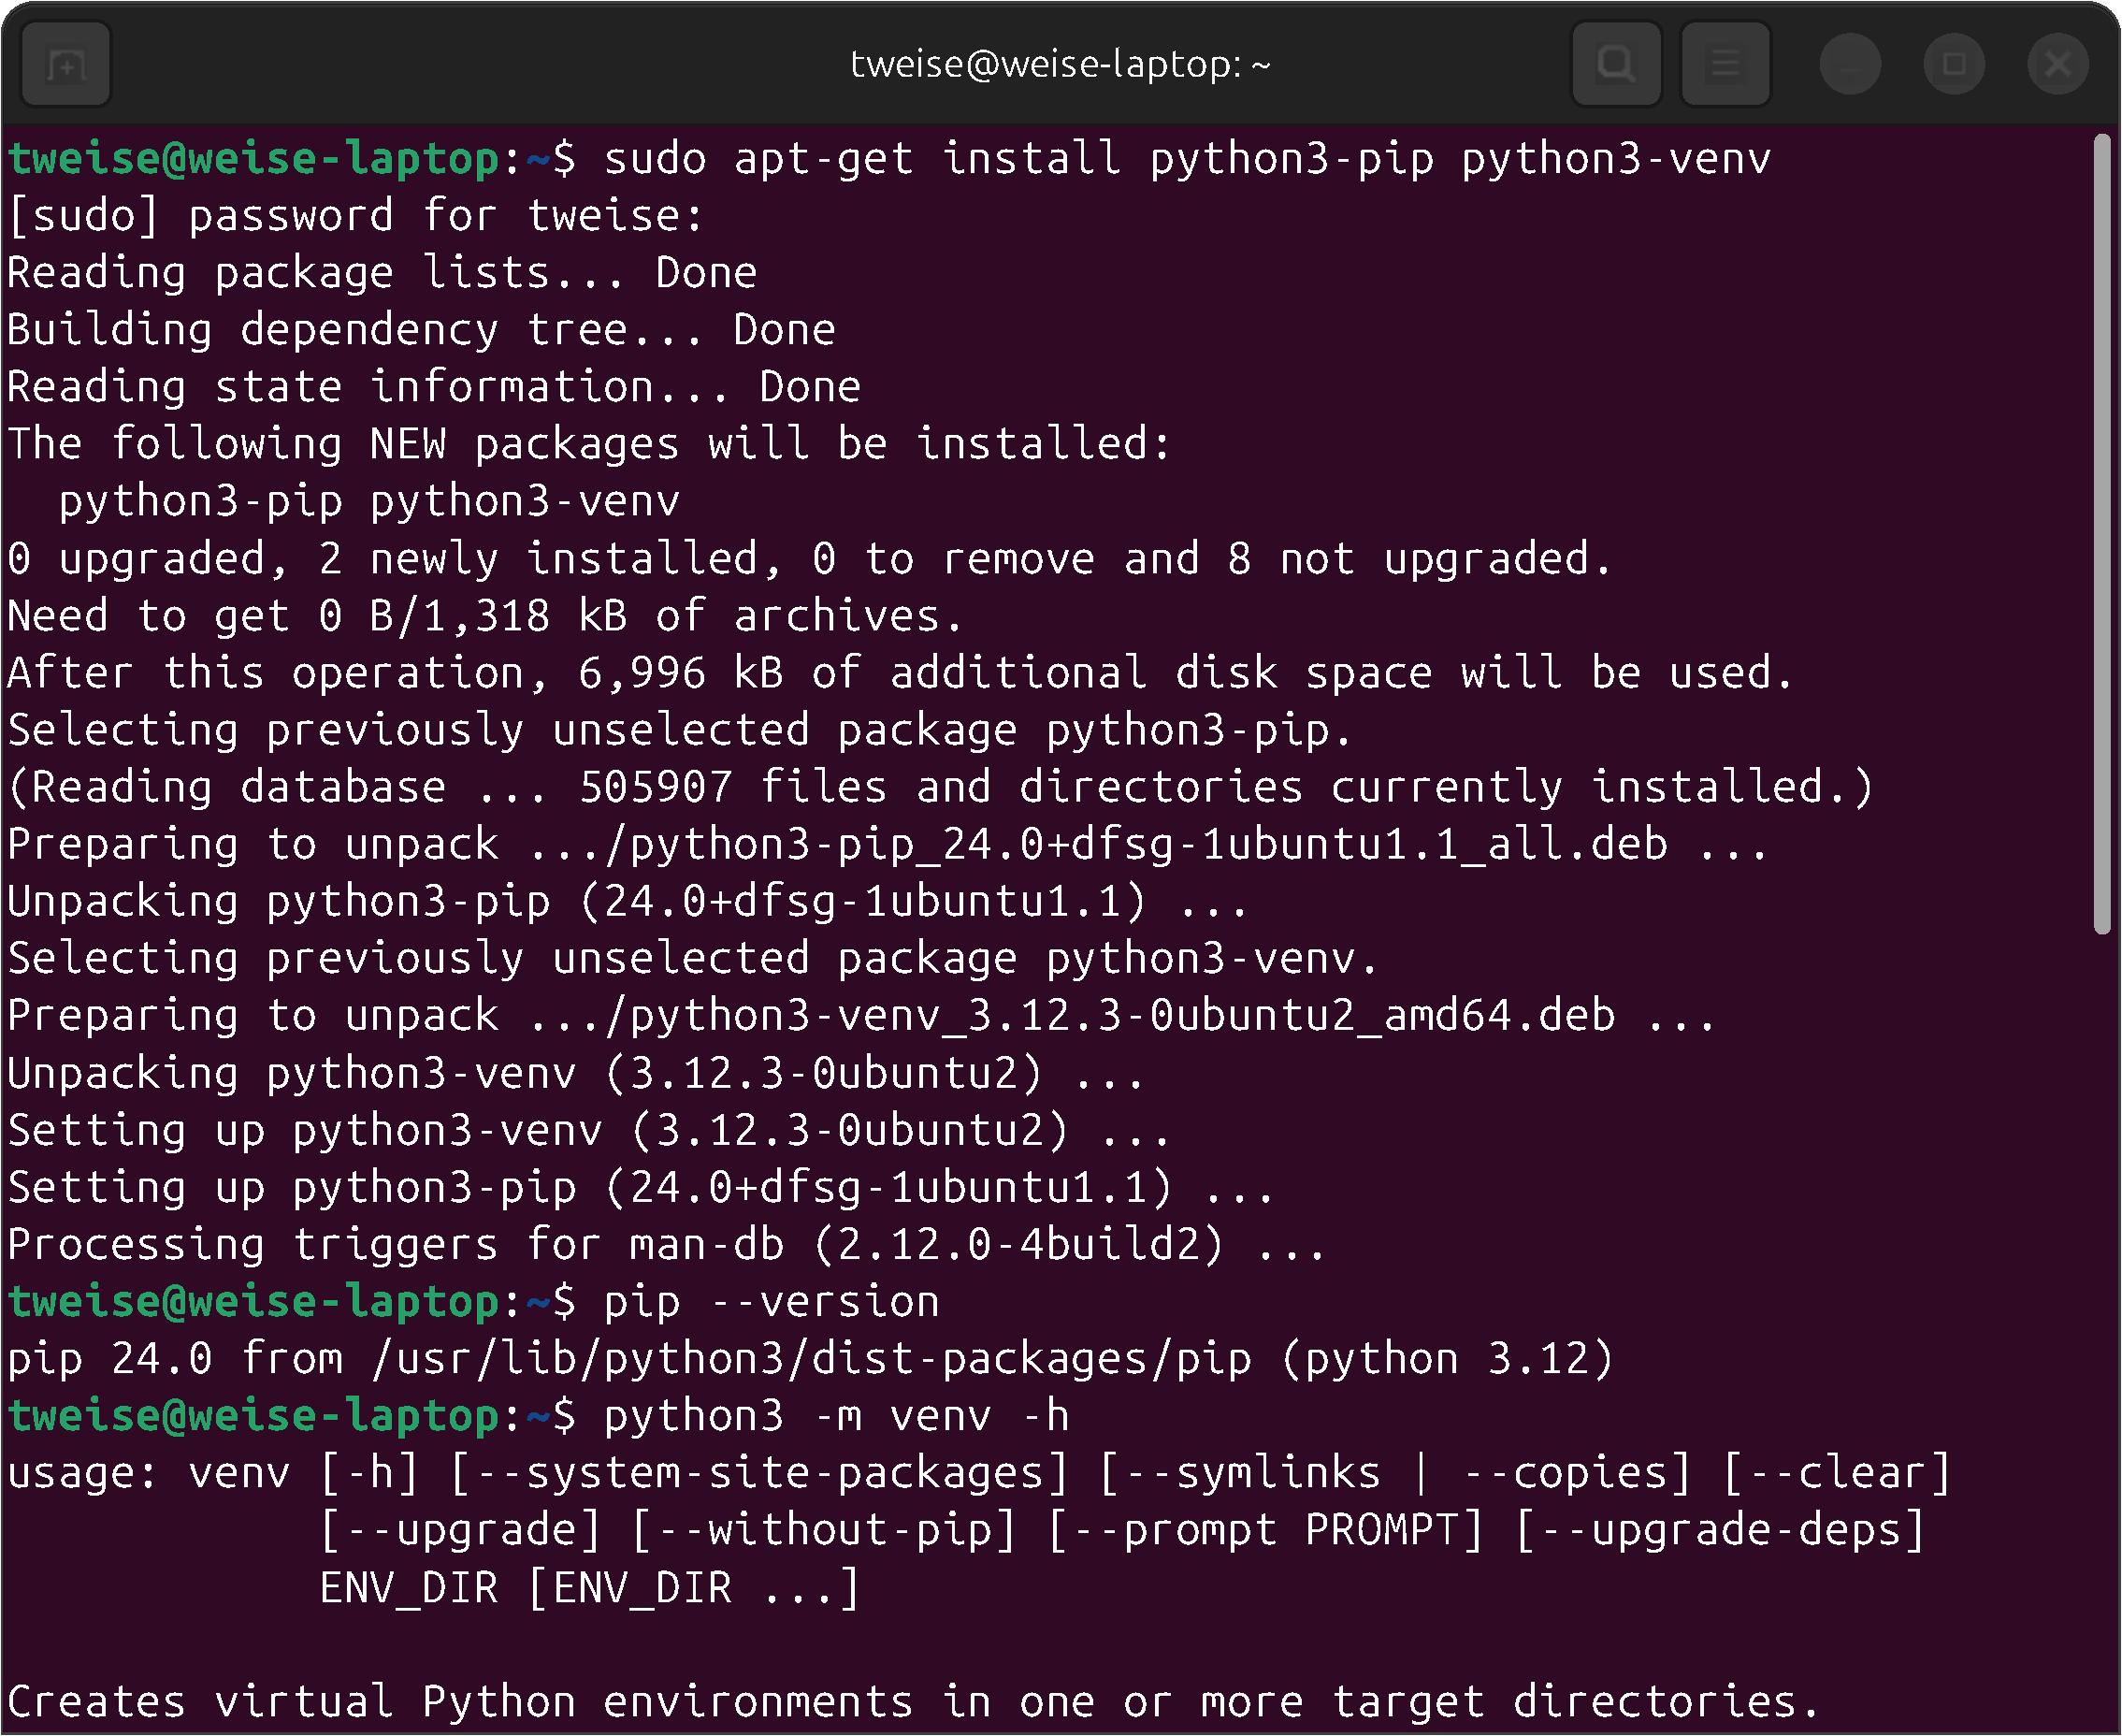
\includegraphics[width=0.7\linewidth]{\currentDir/installPipVenvUbuntu}%
\caption{Installing \pip\ and venv under \ubuntu\ \linux: \pip~is usually already installed, \venv\ maybe or maybe not. %
We need to use the \bashil{apt-get} route to make sure that both \bashil{python3-pip} and \bashil{python3-venv} are installed.}%
\label{fig:installPipVenvUbuntu}%
\end{figure}%
%
First, we need to make sure that both \pip\ and \venv\ are installed.
On some systems, they compare pre-installed with \python~3, which itself comes pre-installed.
On others, at least \venv\ needs to be installed.
These installations need to be managed by the system via \aptGet\ and not~\pip, because \python\ is used for several different things under \ubuntu\ \linux.
Only the \linux\ package manager can make sure that not inconsistencies arise.
We install the packages \bashil{python3-pip} and \bashil{python3-venv} using \aptGet.
This requires superuser privileges, i.e., \pgls{sudo}, so we write \bashil{sudo apt-get install python3-pip python3-venv}.
After entering the password, both packages are installed~(if they are not already installed).
This process is illustrated in \cref{fig:installPipVenvUbuntu}.
After \aptGet\ completes, we can check the version of \pip\ via \bashil{pip --version}.
Whether \venv\ is installed correctly can be checked via \bashil{python3 -m venv -h}.

\gitBashAndOutput{\programmingWithPythonCodeRepo}{10_packages}{numpy_user_venv.sh}{packages:numpy_user_venv}{%
An example of using \pglspl{virtualEnvironment} and \pip\ under \ubuntu\ \linux\ to install \numpy\ and to run our program \cref{lst:packages:numpy_user}.}%
%
\Cref{lst:packages:numpy_user_venv} presents a self-contained example where we execute the necessary commands to setup a \pgls{virtualEnvironment}, install the needed package, run our program, and tear down the virtual environment.
In the real world, you would set up the environment once and could use it many times to run your program.

Assume that we have already opened a \pgls{terminal} by pressing~\ubuntuTerminal\ and that we have entered the directory where our program~\bashil{numpy_user.py} from \cref{lst:packages:numpy_user} is located.
We begin by creating a new empty directory named~\bashil{.venv} in our current directory by \bashil{mkdir -p .venv} command followed by~\keys{\return}.
Inside this directory, we create an empty \pgls{virtualEnvironment} by typing \bashil{python3 -m venv .venv}, again followed by~\keys{\return}.
The directory \bashil{.venv} now should contain a \python\ interpreter as well as all files needed for managing the environment.

The next step is to activate the environment.
If we would type \bashil{python3} right now, we would still be using the system's \python\ interpreter and the packages installed system-wide.
However, we actually want to use the \pgls{virtualEnvironment} instead.
For this, we need to execute \emph{all} the commands in the file \bashil{.venv/bin/activate}.
The simplest way to do this is to just copy all of them into the current \pgls{terminal} as if we had written by hand.
\bashil{source .venv/bin/activate}, confirmed by~\keys{\return} does exactly that.
If you are following this example on your own computer, then after executing this command, the \bash\ prompt (the little text on the left-hand side) changes, showing that now the \pgls{virtualEnvironment} is active.

This means that any call to the \python\ interpreter will, from now on, use the interpreter stored in the \pgls{virtualEnvironment}.
We can also only use packages that were installed there.
If we execute \bashil{pip install --require-virtualenv numpy}, this will install the \numpy\ \pgls{package}.
But it uses the \python\ interpreter and \pgls{package} directory of the activated \pgls{virtualEnvironment}.
So \numpy\ is not installed system-wide, but into the \pgls{virtualEnvironment}.

We can now execute our small program \bashil{numpy_user.py}.
We type \bashil{python3 numpy_user.py} and hit~\keys{\return}.
Indeed, the expected output \textil{look, a numpy array: [1. 2. 3.]} appears in the \pgls{terminal}, as shown in \cref{exec:packages:numpy_user_venv}.
Our program uses the local \numpy\ installation inside the \pgls{virtualEnvironment}.

If this was a more complex and useful application, then this would be the steps to get it ready and usable:
We create the \pgls{virtualEnvironment} exactly once.
Exactly once we need to install all the required \pglspl{package} into it.
Whenever we want to run our application, we would open a new \pgls{terminal}, enter our directory, activate the \pgls{virtualEnvironment}, and then just run the program.
Before closing the \pgls{terminal}, if we want to be tidy, we can deactivate the \pgls{virtualEnvironment} again by executing~\bashil{deactivate}.

To confirm that we really installed \numpy\ only locally and that our program was really using the \pgls{package} installed in the \pgls{virtualEnvironment}, we try to run our program again \emph{after} deactivating the environment.
As you can see in \cref{exec:packages:numpy_user_venv}, this second execution fails:
A \pythonilIdx{ModuleNotFoundError} is raised and the interpreter terminates.%
%
\begin{sloppypar}%
Finally, in our example in \cref{lst:packages:numpy_user_venv}, we delete the \pgls{virtualEnvironment} directory again via~\bashil{rm -rf .venv}.
Normally, you would \emph{not} do this.\footnote{%
I just clean up here because my examples are automatically executed whenever the book is built and I want to avoid that the examples interfer with each other or that, accidentally, some files from the environment land in my \git\ repositories.}%
You do not want to re-create the \pgls{virtualEnvironment} again every time you execute your application.
As said, once you have installed the required \pglspl{package}, you can simply activate the environment and run your program whenever you want.%
\end{sloppypar}%
%
\FloatBarrier%
\endhsection%
%
\hsection{pip and Virtual Environments under \windows}%
%
\begin{figure}%
\centering%
\tightbox{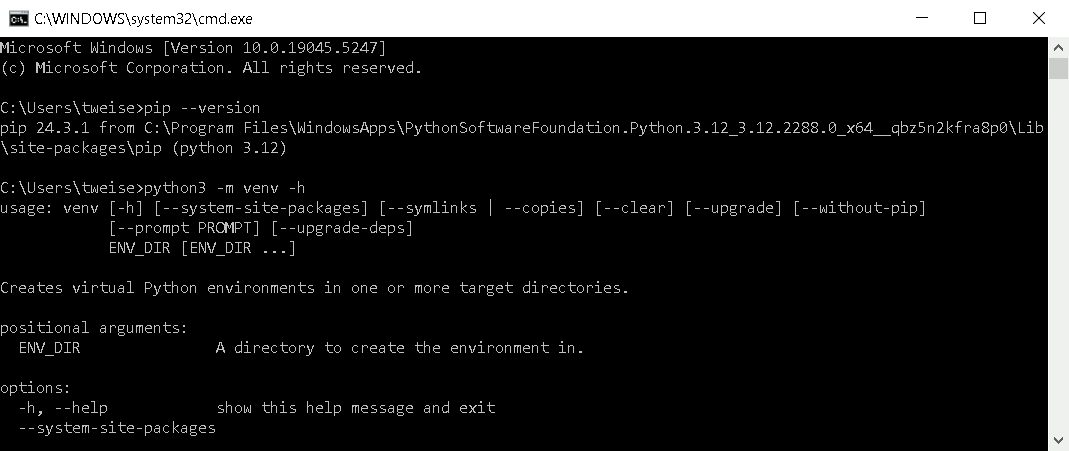
\includegraphics[width=0.85\linewidth]{\currentDir/installPipVenvWindows}}%
\caption{Installing \pip\ and \venv\ under \windows: They are already installed.}%
\label{fig:installPipVenvWindows}%
\end{figure}%
\endhsection%
%
\FloatBarrier%
\endhsection%
%
\endhsection%
%
